\documentclass{article}
\usepackage{graphicx}
\usepackage[style=ieee]{biblatex} % Establecer el estilo de las referencias como IEEE
\usepackage{xcolor}
\usepackage{hyperref}
\usepackage{titletoc}
\usepackage{adjustbox}
\usepackage[spanish]{babel}

\hypersetup{
    colorlinks=true,
    linkcolor=blue, % Color del texto del enlace
    urlcolor=blue % Color del enlace
}

\usepackage{longtable} % Agrega el paquete longtable

\definecolor{mygreen}{RGB}{0,128,0}

\usepackage{array} % Para personalizar la tabla
\usepackage{booktabs} % Para líneas horizontales de mejor calidad
\usepackage{graphicx} % Paquete para incluir imágenes
\usepackage{float}
\usepackage[section]{placeins}

% Definir márgenes
\usepackage[margin=1in]{geometry}

\renewcommand{\contentsname}{\textcolor{mygreen}{Tabla de Contenidos}}

\begin{document}

\begin{titlepage}
    \centering
    % Logo de la Universidad
    
\includegraphics[width=0.48\textwidth]{logo_universidad.png}
    \par\vspace{2cm}

    % Nombre de la Universidad y detalles del curso
    {\Large \textbf{Universidad Nacional de Colombia} \par}
    \vspace{0.5cm}
    {\large Ingeniería de Sistemas y Computación \par}
    {\large 2025966 Lenguajes de Programación (02)\par}
    \vspace{3cm}

    % Detalles del laboratorio y actividad
    {\large \textbf{Taller 1} \par}
    {\large Analizador Léxico\par}
    \vspace{3cm}

    % Lista de integrantes
    {\large \textbf{Integrantes:} \par}
    \vspace{0.5cm}
    \begin{tabular}{ll}
    Javier Andrés Tarazona Jiménez & jtarazonaj@unal.edu.co \\
    - & -@unal.edu.co \\
    \end{tabular}
    \par\vspace{3cm}

    % Fecha
    {\large Junio 24 de 2025 \par}
\end{titlepage}

\tableofcontents % Inserta la tabla de contenidos

\newpage % Salto de página para separar la tabla de contenidos del contenido del documento

% Contenido del artículo----------------------------------------------------------

%---------------------------------------------------------------------------------
% Intro --------------------------------------------------------------------------
%---------------------------------------------------------------------------------

\section{Introducción}\label{sec:intr}

%---------------------------------------------------------------------------------
% Marco Teórico ------------------------------------------------------------------
%---------------------------------------------------------------------------------

\section{Marco Teórico}\label{sec:marc}



\subsection{Contextualización del problema}




%---------------------------------------------------------------------------------
% Descripción y Justificación del Problema a Resolver ----------------------------
%---------------------------------------------------------------------------------

\section{Descripción y Justificación del Problema a Resolver}\label{sec:descr}


\subsection{Objetivo Principal}


%---------------------------------------------------------------------------------
% Diseño de la solución ---------------------------------------------------------
%---------------------------------------------------------------------------------

\section{Diseño de la solución}\label{sec:dis}


La solución se organiza en un pipeline modular de seis capas que separa 
las responsabilidades, el diagrama se puede ver en la imagen \ref{fig:pipelineLexico}.
El \emph{Lector de Archivo} se encarga de la lectura 
del archivo fuente completo, enviado como un .txt. Este es el
un código del lenguaje al que se le quiere pasar el analizador léxico.

A continuación, la \emph{Capa de Preprocesamiento} filtra espacios y tabulaciones 
(o bien lleva la cuenta de líneas cuando se requiera).

La \emph{Capa de Construcción del Lexer} utiliza \texttt{PLY} con banderas 
\texttt{re.VERBOSE} compilando en una sola estructura los patrones de expresión 
regular. Esto facilita el análisis para expresiones de regex
complejas, como las que se usan al combinar
lad funciones de python (fprints) con el propio regex.

El \emph{Motor de Tokenización} recorre la entrada con las reglas definidas y, 
finalmente, en la \emph{Capa de Salida}, se envían los tokens etiquetados 
con su tipo, valor, línea y posición en un archivo de salida, 
listo para las fases posteriores del compilador.

\begin{figure}[ht]
  \centering
  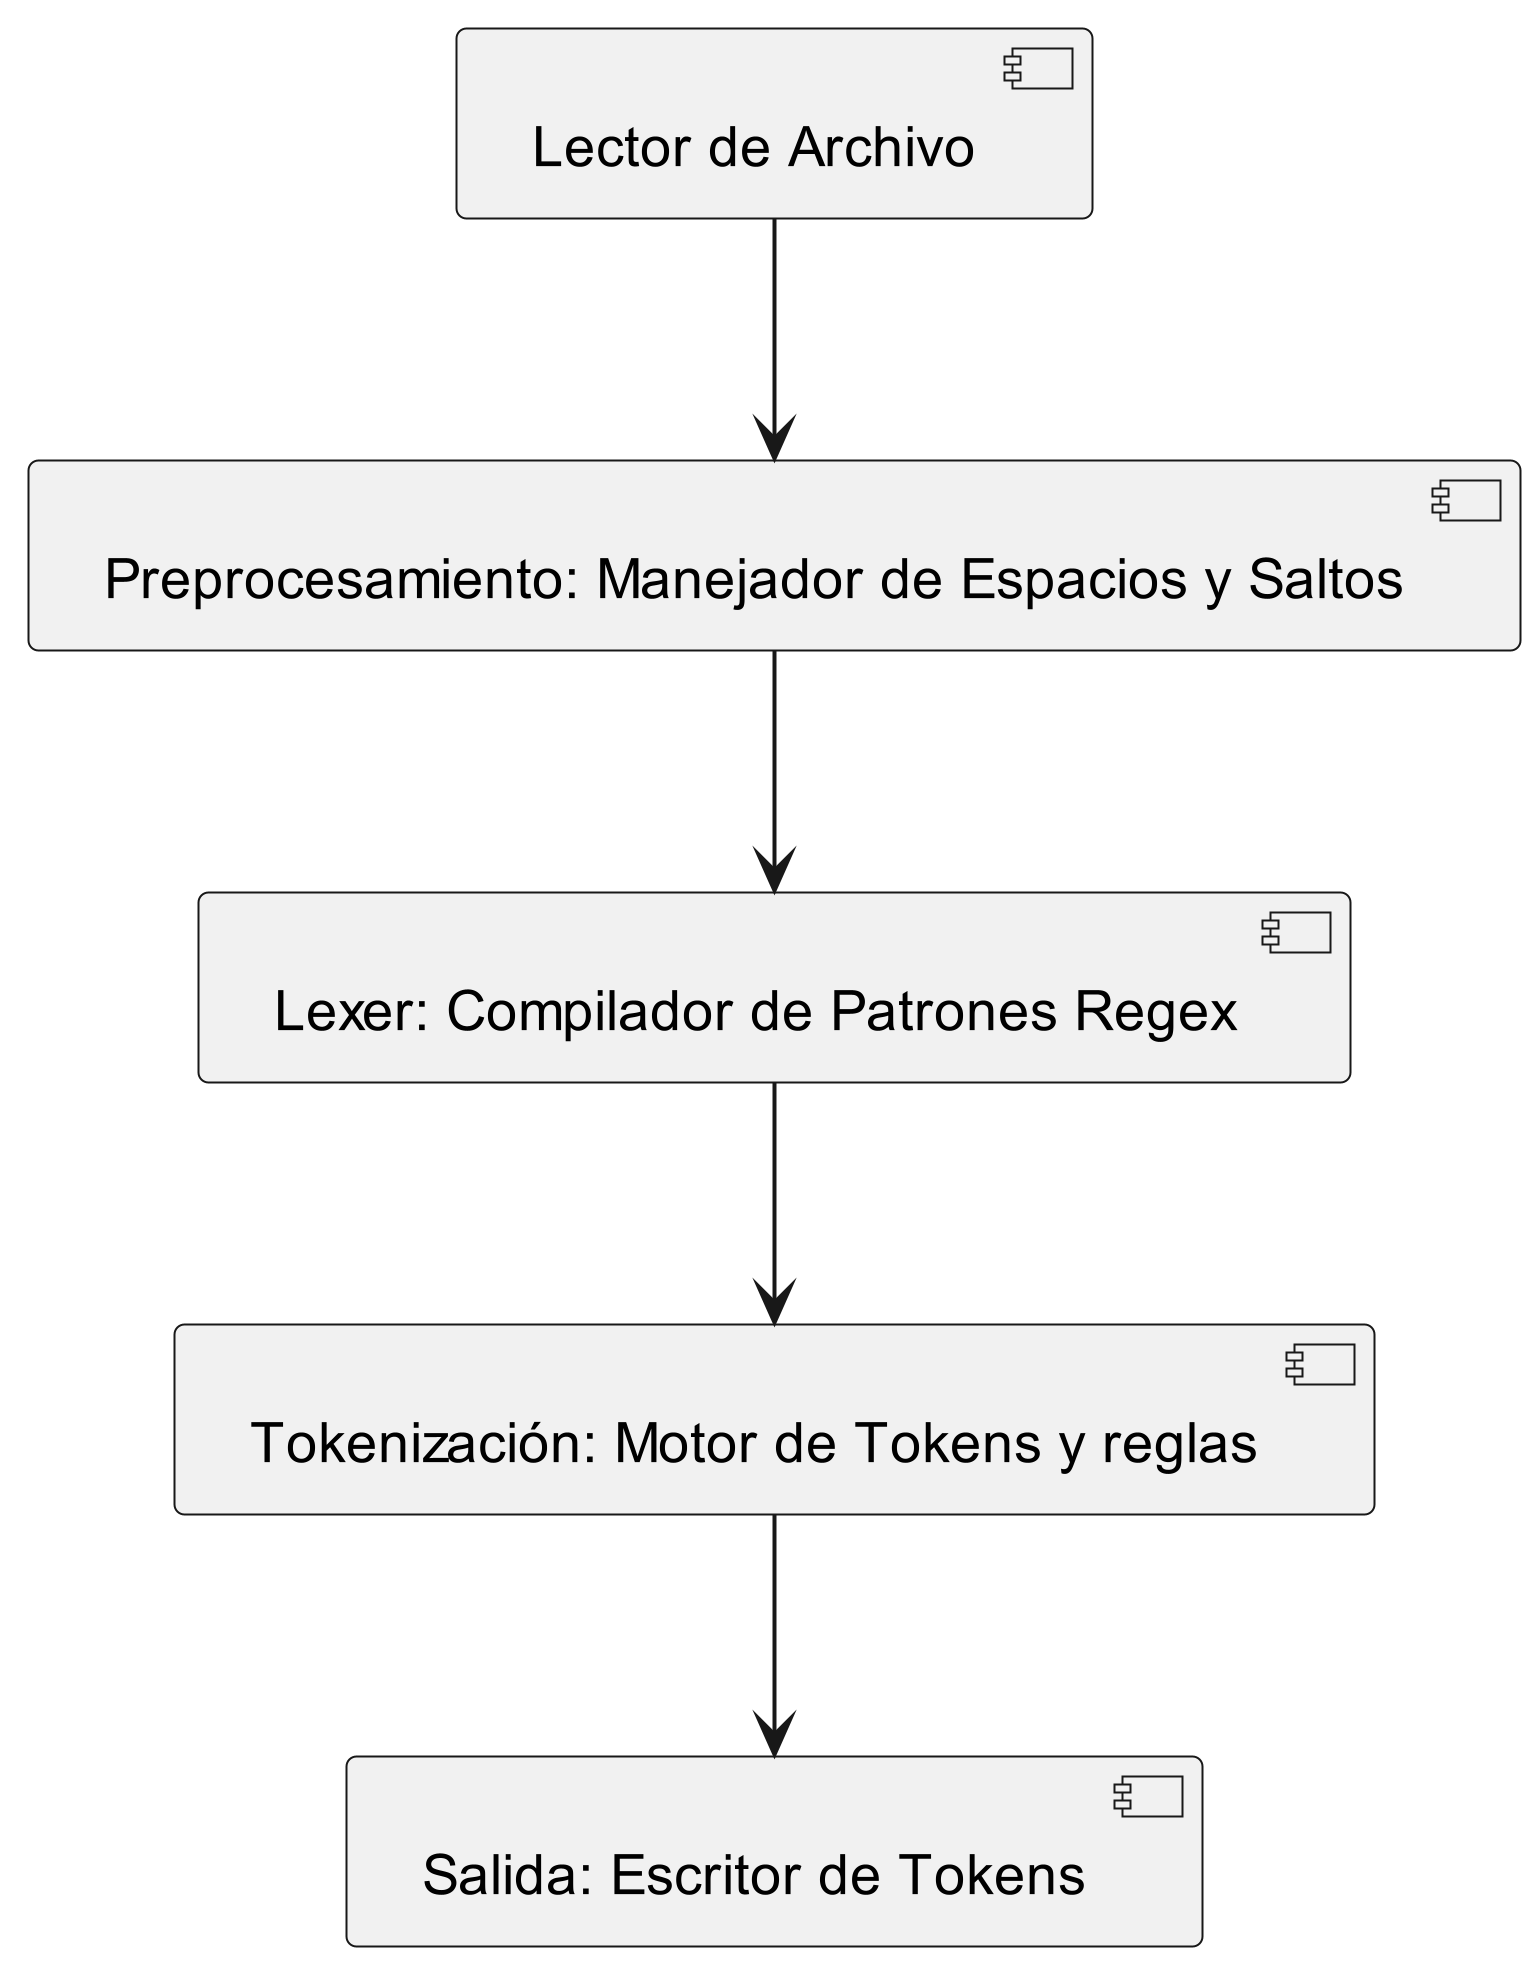
\includegraphics[width=0.7\textwidth]{Flujo.png}
  \caption{Pipeline modular del analizador léxico por capas}
  \label{fig:pipelineLexico}
\end{figure}

\vspace{1em}

En la imagen \ref{fig:MotorTokens1} y \ref{fig:MotorTokens2}
 se pueden ver las categorías léxicas que se implementaron como
reglas del motor de tokens.

\begin{figure}[ht]
  \centering
  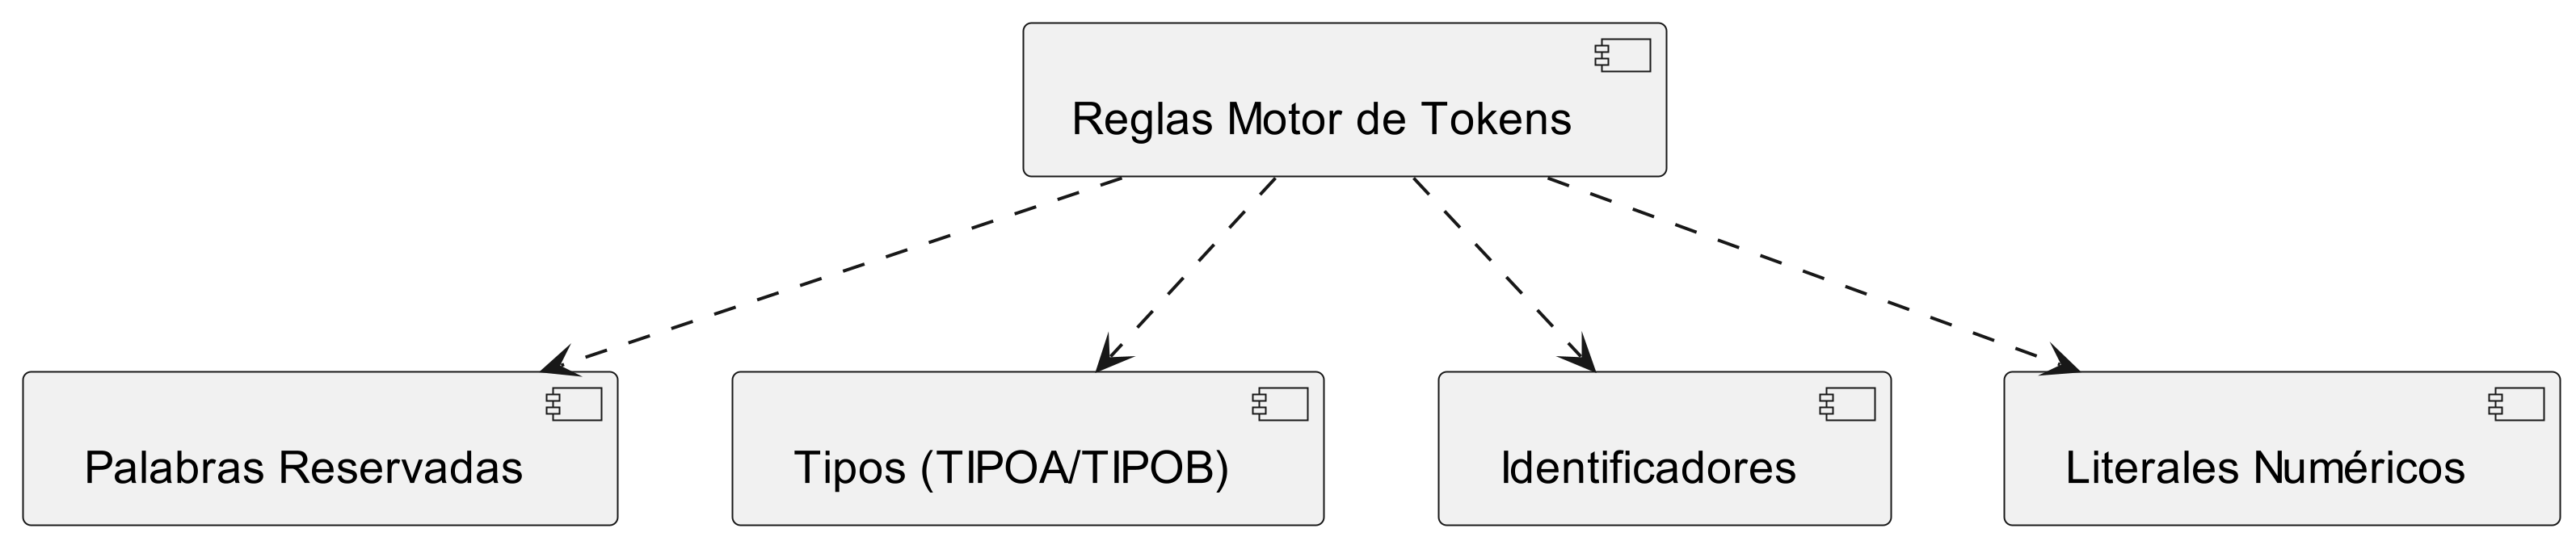
\includegraphics[width=1\textwidth]{MotorTokens1.png}
  \caption{Motor de Tokens Parte 1}
  \label{fig:MotorTokens1}
\end{figure}

\begin{figure}[ht]
  \centering
  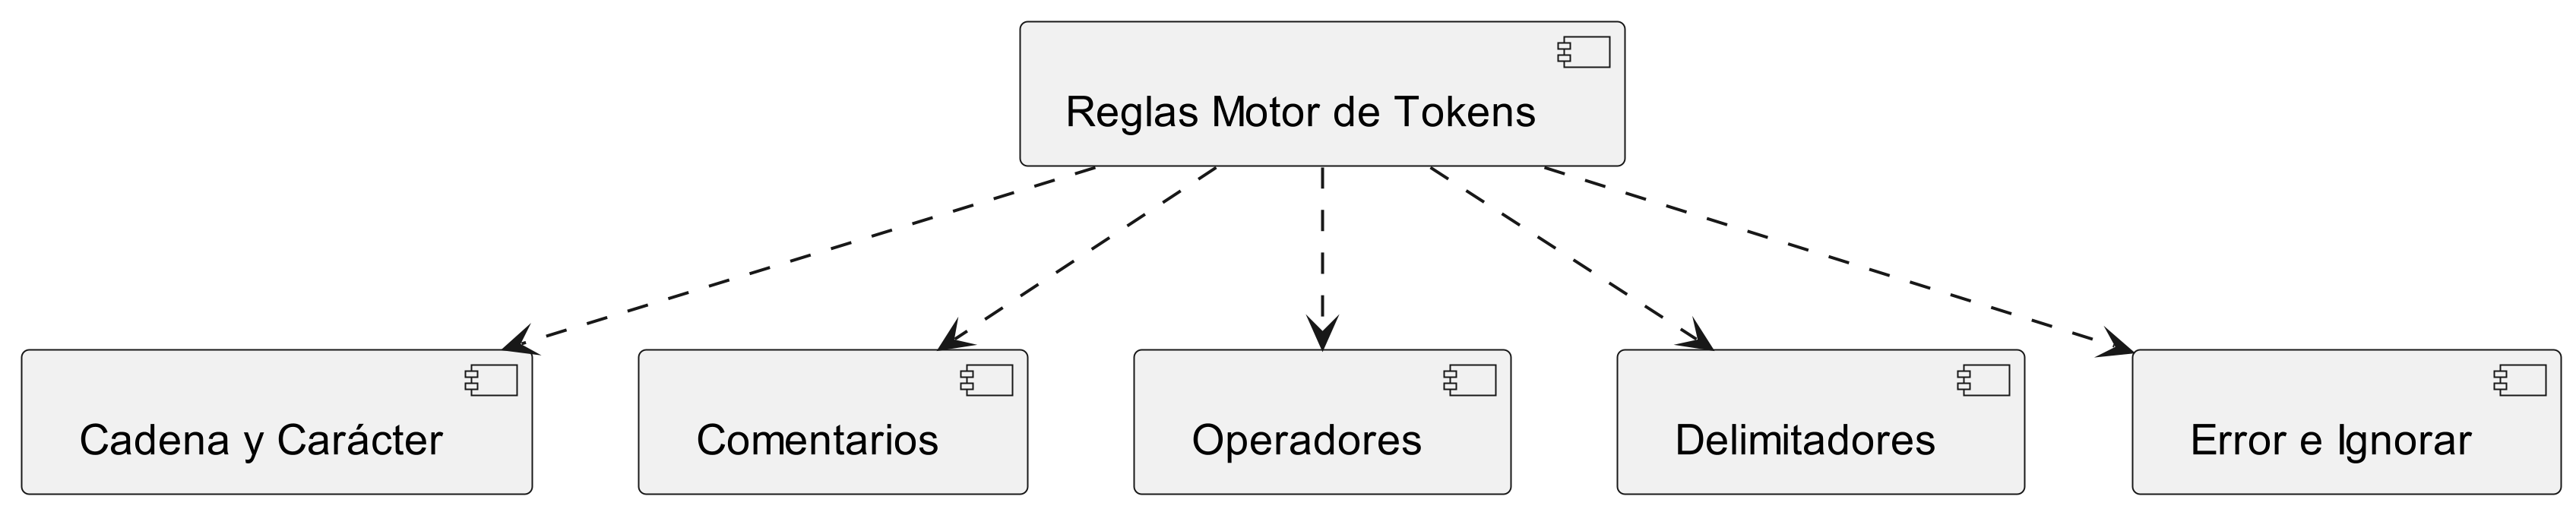
\includegraphics[width=1\textwidth]{MotorTokens2.png}
  \caption{Motor de Tokens Parte 2}
  \label{fig:MotorTokens2}
\end{figure}


\noindent Cada categoría de token se implementa de forma aislada para evitar 
solapamientos:
\begin{itemize}
  \item Las palabras reservadas, \texttt{TIPOA} y \texttt{TIPOB}
      se manejan mediante un único \texttt{t\_ID} que consulta un diccionario 
      \texttt{reserved}, garantizando prioridad a los tipos compuestos 
      (\texttt{Conjunto<T>}, \texttt{MatrizRachas<T>}\dots) antes de clasificar 
      como identificador.
  \item Los literales numéricos aplican precedencia 
      (complejo \(\rightarrow\) real \(\rightarrow\) entero) mediante tres reglas 
        con docstrings, asegurando que expresiones 
        como \texttt{1+2j}, \texttt{3.14e-2} y \texttt{42} se reconozcan correctamente.
  \item Para cadenas y caracteres, se definen patrones robustos 
    que admiten escapes y placeholders (incluyendo soporte para la ñ/Ñ 
    en identificadores), y para comentarios, una regla de función 
    \texttt{t\_COMMENT} captura \texttt{//…} y \texttt{/*…*/} antes de que 
    intervengan los operadores. Se añade que se ponen al inicio para que no 
    se solapen con otras categorías léxicas.
  \item Finalmente, las expresiones de operadores y delimitadores se 
    definen como literales agrupados y ordenados por longitud, 
    evitando ambigüedades gracias al orden de declaración. Por
    ejemplo entre \texttt{!=} y \texttt{!}.
\end{itemize}


%---------------------------------------------------------------------------------
% Código Fuente ---------------------------------------------------------
%---------------------------------------------------------------------------------

\section{Código Fuente}\label{sec:cod}

El código fuente completo de este modelo se encuentra adjunto como 
(Taller1.zip)
y disponible en el repositorio GitHub del proyecto:

\begin{center}
\url{https://github.com/JavierTarazona06/LP02_Tareas/tree/main/taller1/code}
\end{center}

%---------------------------------------------------------------------------------
% Manual Usuario ---------------------------------------------------------
%---------------------------------------------------------------------------------

\section{Manual Usuario}\label{sec:man_u}

El primer paso es descargar el archivo \texttt{Taller1.zip}.

El repositorio contiene:
\begin{itemize}
  \item \textbf{Código principal}
  \begin{description}
    \item[\texttt{a\_lexico.py}] Código principal del analizador léxico: 
      define la lista de tokens, patrones (regex) y funciones \texttt{t\_…} que definen patrones
      para cada categoría, y construye el lexer con PLY.
  \end{description}

  \item \textbf{Otros}
  \begin{description}
    \item[\texttt{InstallationGuide.md}] Guía paso a paso (Markdown) para crear y 
      activar el entorno virtual y luego instalar las dependencias necesarias con 
      \texttt{pip install -r requirements.txt}.
    \item[\texttt{requirements.txt}] Lista de dependencias del proyecto 
      (principalmente la versión de \texttt{ply} necesaria para ejecutar el analizador).
  \end{description}

  \item \textbf{Testing}
  \begin{description}
    \item[\texttt{tests/prototype1.txt}] Primer caso de prueba: un 
      fragmento de código del lenguaje fuente (teoría de rachas) propuesto para verificar el lexer.
    \item[\texttt{tests/prototype1\_lex.txt}] Salida esperada del lexer al 
        procesar \texttt{prototype1.txt}, listando línea:posición, tipo de token y lexema.
    \item[\texttt{tests/prototype2.txt}] Segundo caso de prueba: ejemplo con estructuras de 
        datos (matrices, arreglos) y tipado flotante del lenguaje propuesto.
    \item[\texttt{tests/prototype2\_lex.txt}] Tokens generados por el lexer para el contenido 
        de \texttt{prototype2.txt}.
    \item[\texttt{tests/prototype3.txt}] Tercer caso de prueba: implementación 
        del algoritmo de Euclides en el lenguaje propuesto
    \item[\texttt{tests/prototype3\_lex.txt}] Salida de tokens correspondiente al 
        archivo \texttt{prototype3.txt}.
  \end{description}
\end{itemize}


Una vez descargado, descomprímalo y acceda a la carpeta. Dentro de ella, cree un 
entorno virtual utilizando Python 3.10. o superior. Para ello, ejecute el siguiente 
comando en 
la terminal o línea de comandos:

\begin{itemize}
  \item En Windows:
  \begin{verbatim}
    python3.12 -m venv nombre_del_entorno
  \end{verbatim}
  \item En macOS o Linux:
  \begin{verbatim}
    python3.12 -m venv nombre_del_entorno
  \end{verbatim}
\end{itemize}

Donde \texttt{nombre\_del\_entorno} es el nombre que desea asignar a su entorno virtual. 
A continuación, active el entorno virtual:

\begin{itemize}
  \item En Windows:
  \begin{verbatim}
    .\nombre_del_entorno\Scripts\activate
  \end{verbatim}
  \item En macOS o Linux:
  \begin{verbatim}
    source nombre_del_entorno/bin/activate
  \end{verbatim}
\end{itemize}

Asegúrese de tener el entorno virtual activado. 
A continuación, descargue las dependencias necesarias 
(en este caso, únicamente \texttt{PLY} para gestionar \texttt{Lex}):

\begin{verbatim}
    pip install -r requirements.txt
\end{verbatim}

Una vez activo y el entorno instalado, puede ejecutar el archivo 
principal con el siguiente comando:

\begin{center}
  \begin{adjustbox}{minipage=\linewidth, center}
  \begin{verbatim}
    python a_lexico.py
  \end{verbatim}
  \end{adjustbox}
\end{center}

\begin{enumerate}
  \item Al iniciar el analizador, la terminal mostrará el prompt:
    \begin{verbatim}
      term>
    \end{verbatim}
    y permanecerá a la espera de que se introduzca la ruta completa (\texttt{path}): 
    la dirección, el nombre y la extensión del archivo fuente que contiene 
    el código en el lenguaje propuesto.
    \\
    \textbf{Ejemplo:}
    \begin{verbatim}
      term> C:\proyectos\mi_codigo.txt
    \end{verbatim}

    Cabe resaltar que no toca especificar el path, si el archivo
    se encuentra en current directory.

  \item Una vez recibida la ruta, el analizador léxico leerá y procesará ese archivo.

  \item A continuación, generará un archivo de salida en el \emph{mismo directorio},
    con el \emph{mismo nombre} que el original y el sufijo \_\texttt{lex.txt}.
    \\
    \textbf{Si el archivo de entrada es}
    \begin{verbatim}
        C:\proyectos\mi_codigo.txt
    \end{verbatim}
    \textbf{el analizador creará}
    \begin{verbatim}
      C:\proyectos\mi_codigo_lex.txt
    \end{verbatim}

  \item El contenido de \texttt{mi\_codigo\_lex.txt} 
    será el análisis léxico completo. Cada línea incluirá:
    \begin{itemize}
      \item \textbf{Posición}: por ejemplo, línea:columna o un offset numérico.
      \item \textbf{Tipo de token}: por ejemplo, \texttt{ID}, \texttt{ENTERO}, \texttt{PALABCLAVE}.
      \item \textbf{Lexema}: el texto exacto reconocido.
    \end{itemize}
    \textbf{Ejemplo de línea de salida:}
    \begin{verbatim}
      3:15    ID        contador
      3:23    OPARIT    =
      3:25    ENTERO    42
    \end{verbatim}
\end{enumerate}

%---------------------------------------------------------------------------------
% Manual Técnico ---------------------------------------------------------
%---------------------------------------------------------------------------------

\section{Manual Técnico}\label{sec:man_t}



%---------------------------------------------------------------------------------
% Experimentación ---------------------------------------------------------
%---------------------------------------------------------------------------------

\section{Experimentación}\label{sec:exp}

\subsection{Análisis de resultados}

\subsubsection{Escenario 1: }

\subsubsection{Escenario 2: }
 
\subsubsection{Escenario 3: }



\section{Referencias}
\renewcommand{\refname}{}

\begin{thebibliography}{9}

\bibitem{ref} \label{ref:lexPy1} J. R. Levine, T. Mason, and D. 
Brown, “Lex \& Yacc,” 2nd ed., O’Reilly \& Associates, 1992.

\bibitem{ref} \label{ref:lexPy2}  D. M. Beazley, “PLY (Python Lex‐Yacc)
Manual,” Version 3.11, 2023. [Online]. Available: https://www.dabeaz.com/ply/.

\bibitem{ref} \label{ref:rachas} J.~E.~Ortiz~Triviño, ``Lenguaje para 
  procesamiento de rachas,'' Documento interno, Universidad Nacional de 
    Colombia, enviado por correo electrónico, 6 de mayo de 2025.

\end{thebibliography}

\end{document}